\if c\LaTeXe
\quad
\else

\documentclass{article}

\usepackage{amsmath, amssymb}
\usepackage{comment}
\usepackage{graphicx}
%\usepackage[T1]{fontenc}
%\usepackage{ae, aecompl}
\usepackage[numbers]{natbib}

%%%%%%%%%%%%%%%%%%%%%%%%%%%%%%%%%%%%%%%%%%%%%%%%%%%%%%%%%%%%%%%%%%%%%%%%
%% math

%
% General
%

\DeclareMathOperator{\argmin}{arg\,min}
\DeclareMathOperator{\argmax}{arg\,max}

%
% Sets
%

\newcommand{\card} [1]{{\lvert #1 \rvert}}
\newcommand{\range}[1]{{\left\{ 1, \dots, #1 \right\}}}

%
% Linear algebra
%

\newcommand{\mat}  [1]{{\bf #1}}
\newcommand{\norm} [1]{{\lVert #1 \rVert}}
\newcommand{\vect} [1]{{\mbox{\boldmath $#1$}}}

%
% Probability. The CTAN `proba` package doesn't seem to be that good.
% TODO ensuremath does not seem to be a good idea.
%

\newcommand{\E}    [2]{{\textrm{E} \left[ #1 \mid #2 \right]}}
\newcommand{\LL}   [2]{{\ensuremath{ L \left( #1 \,\middle|\, #2 \right) }}}
\newcommand{\LLL}  [2]{{\ensuremath{ l \left( #1 \,\middle|\, #2 \right) }}}
\newcommand{\N}    [1]{{\ensuremath{ \# \left( \textrm{ #1 } \right) }}}
\newcommand{\PO}   [1]{{\Pr \left( #1 \right)}}
\newcommand{\PP}   [2]{{\PO{ #1 \,\middle|\, #2 }}}

%%%%%%%%%%%%%%%%%%%%%%%%%%%%%%%%%%%%%%%%%%%%%%%%%%%%%%%%%%%%%%%%%%%%%%%%
%% Theoretical computer science

%
% Computational complexity
%

\DeclareMathOperator{\bigO}{O}
\providecommand{\OO}[1]{\bigO\bigl(#1\bigr)}

%%%%%%%%%%%%%%%%%%%%%%%%%%%%%%%%%%%%%%%%%%%%%%%%%%%%%%%%%%%%%%%%%%%%%%%%
%% General text

% \emph toggles italics; \textit sets italics; \em is deprecated
\newcommand{\term} [1]{{\emph{#1\/}}} 

% We don't need to do append a ~ or \ because TeX already handles .,
% correctly. TODO figure out if italics are correct here
\newcommand{\foreign}[1]{{\textit{#1}}}
\newcommand{\ea}      {{\foreign{et~al.}}}
\newcommand{\eg}      {{\foreign{e.g.}}}
\newcommand{\ie}      {{\foreign{i.e.}}}
\newcommand{\TODO} [1]{{\textbf{TODO}: \textit{#1}}}

%%%%%%%%%%%%%%%%%%%%%%%%%%%%%%%%%%%%%%%%%%%%%%%%%%%%%%%%%%%%%%%%%%%%%%%%
%% Remarks. Collected from the pervasive but untraceable `remarks.tex`.

\newif\ifremark
\long\def\remark#1{
\ifremark%
    \begingroup%
    \dimen0=\columnwidth
    \advance\dimen0 by -0.25in%
    \setbox0=\hbox{\parbox[b]{\dimen0}{\protect\em\textcolor{red}{#1}}}
    \dimen1=\ht0\advance\dimen1 by 2pt%
    \dimen2=\dp0\advance\dimen2 by 2pt%
    \vskip 0.25pt%
    \hbox to \columnwidth{%
        \vrule height\dimen1 width 3pt depth\dimen2%
        \hss\copy0\hss%
        \vrule height\dimen1 width 3pt depth\dimen2%
    }%
    \endgroup%
\fi}

\newcommand{\remarkname}[2] {
    \remark{{\bf #1}:#2}
}


\begin{document}

\fi

\section{Linear Regression + EM-like alternate update}
\subsection{Overview}
The goal of the algorithm is to find a low-rank approximation of the sparse rating matrix
\begin{equation}
R \approx MU
\end{equation}
where $M$ is a $n_M$-by-$d$ movie property matrix, $U$ is a
$d$-by-$n_U$ user property matrix, and $d$ is the dimension of the
low-rank approximation. Due to the missing entries of $R$, $M$ and $U$
cannot be obtained from singular value decomposition. Instead, the
algorithm learns $M$ and $U$ using linear regression and an EM-like
alternate update algorithm.

The time and space complexity of the algorithm is proportional to the data size $(n_U+n_M)$, so it is tractable even for the huge data set of Netflix Prize. However, it badly overfits to the training data especially when the rating matrix is sparse.

\subsection{Learning Algorithm}

At the beginning of the algorithm, $M$ is randomly initialized and fixed. Then the $i$th column of $U$ is learned by regular linear regression as follows;
\begin{equation}
\vect{u}_i=(\check{M}^T\check{M})^{-1}\check{M}^T \check{\vect r}_i \label{eq:lrem_core}
\end{equation}
where $\check{\vect r}_i$ is a column vector constructed from the $i$th column of the rating matrix $R$, by excluding the missing elements from it. For example, if the $i$th column of $R$ is $[2 \quad \circ \quad 4 \quad \circ \quad \circ \quad 5 \quad \circ]^T$ where``$\circ$'' means missing element, then $\check{r}_i = [2 \quad 4 \quad 5]^T$. $check{M}$ is a matrix with the corresponding rows of $M$.

Then in the next step, $U$ is fixed and each row of $M$ is updated in the exactly same manner. These steps are repeated and U and M are alternatively updated until the training RMSE converges, just as EM algorithm. 

The important fact is that, by repeating this iteration, the training RMSE monotonically decreases, and eventually converges to the (local) optimum. Linear regression finds the parameter which minimizes the log likelihood given the following normal distribution with arbitrary fixed variance $\sigma^2$;
\begin{equation}
r_{i,j}\sim N(\vec{m}_i \cdot {\vect u}_j, \sigma^2)
\end{equation}
where $\vec{m}_i$ is the $i$ th row of $M$ and ${\vect u}_j$ is $j$ th column of $U$.

Thus, just as EM algorithm, the log likelihood of the training data monotonically decreases in each iteration. With $\sigma = 1/\sqrt{2}$, the RMSE is exactly the same as the log likelihood. Thus the training RMSE monotonically decreases by iterations.

\subsection{Estimation}
Given the trained matrices $U$ and $M$, the maximum likelihood estimation of the ratings can be easily obtained as follows;
\begin{equation}
\hat{r}_{i,j}=\vec{m}_i \cdot {\vect u}_j.
\end{equation}

Although the actual ratings are given as integer numbers from one to five, the estimations by this algorithm are real numbers. We use the real number outputs without rounding them. However, since ratings are from one to five, the estimations above five are turned into five, and those below one are turned into one. %We call it \textit{rating range correction}\footnote{Is there more appropriate name for this....??}.

\subsection{Result}

The algorithm is implemented with MATLAB and worked successfully.

Since the initial value of $M$ is randomly chosen, the result is stochastic. In fact it appears that the result is very sensitive to the initial value of $M$. Figure \ref{fig:lrem_typical_plot.eps} shows the typical result of the training RMSE and the test RMSE as well as the RMSE when the estimation is simply the average rating of each movie (i.e. zero-order estimation). The training RMSE monotonically decreases over iterations as we expected, but test RMSE does not necessarily monotonically decreases. There is a large gap between training RMSE and test RMSE, indicating that the algorithm badly overfits to the training data.

\begin{figure}[ht]
  \begin{center}
    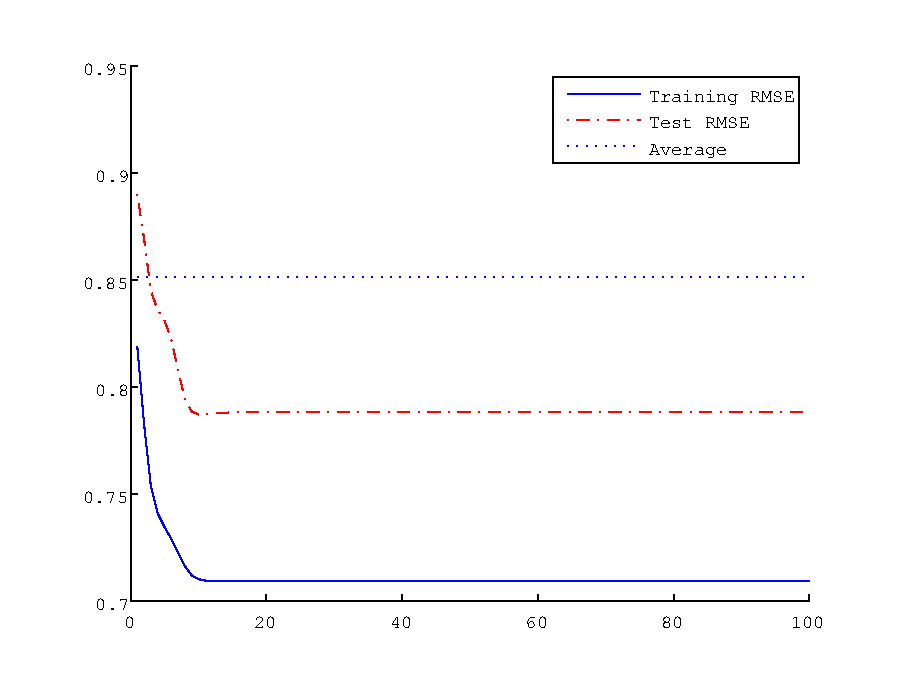
\includegraphics[scale=0.7]{figure/lrem_typical_plot.eps}
  \end{center}
  \caption{Typical result when $d = 2$ and (Ratio of missing element)=0.5. The dotted line shows the RMSE when the estimation is simply the average rating of each movie (i.e. zero-order estimation)}
  \label{fig:lrem_typical_plot.eps}
\end{figure}

Table \ref{table:lrem_result} compares the average RMSE of ten runs with different dimensions of the low-rank approximation $d$ and different ratio of the missing element in the rating matrix. Looking at the table in column-wise, it is found that the algorithm works better for the raining data with less missing ratings, which is an obvious result. An interesting result can be found by looking at the table in row-wise; larger dimension results in the larger RMSE when the rating matrix is sparse, while it results in the smaller RMSE when the rating matrix is mostly filled. It is because the algorithm badly overfits to the training data when the number of free parameters are large while the number of the available training data is small. 


\begin{table}[ht]
 \caption{RMSE with different dimensions $d$ and different ratio of the missing element. The values are the average of ten runs.}
 \label{table:lrem_result}
 \begin{center}
  \begin{tabular}{|c|c||c|c|c|}
    \hline
    \multicolumn{2}{|c|}{}  & \multicolumn{3}{|c|}{Ratio of missing element in $R$} \\
    \cline{3-5}
     \multicolumn{2}{|c|}{}    &  0.7  &  0.5  & 0.2   \\
    \hline
    \hline
       & 1 &  0.808  &  0.795  &  0.789  \\
    \cline{2-5}
     $d$ & 2 &  0.859  &  0.790  & 0.772   \\
    \cline{2-5}
     & 3 &  0.933  &  0.808  &  0.772  \\
    \hline
  \end{tabular}
 \end{center}
\end{table}

\subsection{Complexity Analysis}
\paragraph{Time complexity} 
The most time consuming part of the algorithm is the $d$ by $d$ matrix inversion $(\check{M}^T\check{M})^{-1}$ in Eq. \ref{eq:lrem_core}. In practice, Gauss Elimination, which has a complexity of $\OO{n^3}$, is used to find the solution instead of complete matrix inversion. The inverse of matrix is computed $(n_U+n_M)$ times in each iteration. Thus the time complexity of the algorithm is 
\begin{equation}
\OO{d^3N(n_U+n_M)}
\end{equation}
where $N$ is the number of iterations.

\paragraph{Space complexity}
Only $U$ and $M$ are stored during computation. Thus the space complexity is
\begin{equation}
\OO{d(n_U+n_M)}.
\end{equation}

\subsection{Estimated performance on the full Netflix Prize data}
\paragraph{Computational cost}
It took about 15 seconds for 100 iteration with $n_U=892$, $n_M=51$, and $d=3$ on Intel Celeron 2.0 GHz CPU. Thus for the full data set of Netflix Prize where $n_U=480,189$ and $n_M=17,770$, the computation for 100 iterations would take about 2 hours with $d=3$. Requied memory space would be about 11 MByte. Thus this is a tractable algorithm for the full Netflix Prize data.

\paragraph{RMSE}
In the actual Netflix prize data 99.9\% elements of the rating matrix are missing. With the small data set where $n_U=892$, $n_M=51$, the algorithm cannot run with 99.9\% sparsity since $(\check{M}^T\check{M})^{-1}$ in Eq. \ref{eq:lrem_core} become singular for most of the rows due to the lack of data. One thing we can say for sure from Table \ref{table:lrem_result} is that RMSE would be worse than 0.808 for the full Netflix prize data. Trying the algorithm on full data is the future work.



\if c\LaTeXe
\quad
\else
\end{document}
\fi



